\chapter{Design Of the System}\label{chap4}
\newpage
\section{Requirement Engineering}
\subsection{Requirement Elicitation}
Requirements were gathered from meetings with the project guide, discussions with a collaborating clinician, the drug labels and guidelines used for the safety rules, the team's dataset review and variable-selection notes (September 2026), and the literature in Chapter~\ref{chap2}. They were written as numbered, testable statements following the ISO/IEC/IEEE 29148 style.

\subsection{Software lifecycle model}
The project follows an incremental, iterative model with one-week sprints and a review gate at the end of each week. Each increment ends with working, tested software: the causal engine and the phone website for the mid-semester review (30 September), the RAG layer (9 and 16 October), integration and evaluation (23 October) and the final version (30 October). A waterfall model would leave all integration risk to the end; the automated safety tests (168 at present) act as a gate on every increment, and continuous integration runs them on Linux, macOS and Windows for every change.

\subsection{Requirement Analysis}
\begin{longtable}{p{1.1cm}p{9.6cm}>{\raggedright\arraybackslash}p{3.3cm}}
\caption{Functional requirements and their status on 26 September 2026}\label{tab:fr}\\\toprule
ID & Requirement & Status\\\midrule\endhead
FR1 & Capture age, sex, diabetes duration, BMI, baseline HbA1c (\%), eGFR (mL/min/1.73m$^2$), cardiovascular disease, heart failure, past hypoglycaemia, ketoacidosis, pancreatitis, type 1 diabetes and cost concern. & Done\\
FR2 & Validate inputs and units; reject out-of-range values with a clear message. & Done\\
FR3 & Apply the cited safety rules and show every exclusion or caution with its reason and source. & Done (10 rules)\\
FR4 & Compute generalised propensity scores and an overlap check for each remaining option. & Done\\
FR5 & Show ``insufficient evidence'', with the reason, when overlap is too low. & Done\\
FR6 & Estimate each allowed option's six-month HbA1c change with a 95\% interval. & Done\\
FR7 & Show hypoglycaemia risk and weight change with intervals. & In progress\\
FR8 & Look up the monthly cost (INR) from a dated, cited price table. & Done; prices await confirmation\\
FR9 & Show a cited explanation from licence-cleared sources only. & Retrieval done; writer in October\\
FR10 & Log every request: model and rule versions, statuses and rule IDs (never patient values). & Done\\
FR11 & Export a consultation summary. & In progress\\
FR12 & Sign-up, authenticator-app sign-in and admin approval for evaluators. & Done\\\bottomrule
\end{longtable}

\begin{table}[H]\centering\small\caption{Non-functional requirements}\label{tab:nfr}
\begin{tabularx}{\textwidth}{p{3.2cm}Y}\toprule
Quality & Requirement\\\midrule
Clinical safety & All eight safety rules enforced by automated tests\\
Correctness & Estimator tests against known true effects on synthetic data\\
Performance & Under 3 seconds per request on a laptop (the website answers on the phone itself)\\
Availability & Demo-grade; installable website that works offline, plus a recorded demo\\
Security & HTTPS, sign-in with an authenticator app, admin approval, strict content-security policy\\
Privacy & No identifiable patient data; patient details never leave the device; principles of India's DPDP Act, 2023\\
Auditability & Append-only log of every request\\
Usability & System Usability Scale score of at least 68 \cite{brooke1996}\\
Accessibility & WCAG 2.1 AA for the web interface\\
Maintainability & Readable, typed Python; every module tested\\
Licence compliance & Every knowledge source recorded with its licence category\\\bottomrule
\end{tabularx}\end{table}

\subsubsection{UML diagrams/ DFDs based on the project}
\begin{figure}[H]\centering
\resizebox{\ifdim\width>\textwidth\textwidth\else\width\fi}{!}{\begin{tikzpicture}[>=Stealth,font=\small,ent/.style={draw,minimum width=2.6cm,minimum height=0.9cm},store/.style={draw,minimum width=2.8cm,minimum height=0.8cm}]
\node[draw,circle,minimum size=2.4cm,align=center] (S) at (0,0) {0\\DiaCausal};
\node[ent] (C) at (-6.5,0) {Clinician};
\node[store] (G) at (0,2.8) {Guideline documents};
\node[store] (A) at (5.5,0) {Audit log};
\draw[->] ([yshift=6pt]C.east) -- node[above,font=\footnotesize,pos=0.4]{patient details} ([yshift=6pt]S.west);
\draw[<-] ([yshift=-6pt]C.east) -- node[below,font=\footnotesize,pos=0.4]{options, ranges, reasons} ([yshift=-6pt]S.west);
\draw[->] (G) -- node[right,font=\footnotesize]{passages} (S);
\draw[->] (S) -- node[above,font=\footnotesize]{record} (A);
\end{tikzpicture}}\caption{Data flow diagram, level 0}\label{fig:dfd0}\end{figure}

\begin{figure}[H]\centering
\resizebox{\ifdim\width>\textwidth\textwidth\else\width\fi}{!}{\begin{tikzpicture}[>=Stealth,font=\footnotesize,proc/.style={draw,rounded corners,minimum width=2.5cm,minimum height=1cm,align=center},store/.style={draw,minimum width=2.2cm,minimum height=0.6cm}]
\node[proc] (p1) at (0,0) {1\\Validate input};
\node[proc] (p2) at (3.4,0) {2\\Safety rules};
\node[proc] (p3) at (6.8,0) {3\\Causal engine};
\node[proc] (p4) at (10.2,0) {4\\Cost lookup};
\node[proc] (p5) at (10.2,-2.4) {5\\Cited evidence\\(RAG)};
\node[proc] (p6) at (6.8,-2.4) {6\\Log and display};
\node[store] (r) at (3.4,1.6) {rules.csv};
\node[store] (m) at (6.8,1.6) {fitted model};
\node[store] (pr) at (10.2,1.6) {prices.csv};
\node[store] (co) at (13.1,-2.4) {corpus};
\draw[->] (p1)--(p2); \draw[->] (p2)--(p3); \draw[->] (p3)--(p4); \draw[->] (p4)--(p5); \draw[->] (p5)--(p6);
\draw[->] (r)--(p2); \draw[->] (m)--(p3); \draw[->] (pr)--(p4); \draw[->] (co)--(p5);
\end{tikzpicture}}\caption{Data flow diagram, level 1}\label{fig:dfd1}\end{figure}

\begin{figure}[H]\centering
\resizebox{\ifdim\width>\textwidth\textwidth\else\width\fi}{!}{\begin{tikzpicture}[font=\footnotesize,uc/.style={draw,ellipse,minimum width=4.6cm,minimum height=0.72cm}]
\draw[rounded corners] (2.8,1.4) rectangle (9.2,-6.1); \node at (6,1.1) {\textbf{DiaCausal}};
\node[align=center] (cl) at (0,-0.9) {\Large$\bigcirc$\\Clinician};
\node[align=center] (ev) at (0,-3.2) {\Large$\bigcirc$\\Evaluator};
\node[align=center] (ad) at (0,-5.1) {\Large$\bigcirc$\\Administrator};
\node[uc] (u1) at (6,0.3) {Sign up / sign in with code};
\node[uc] (u2) at (6,-0.6) {Enter patient details};
\node[uc] (u3) at (6,-1.5) {Compare the three options};
\node[uc] (u4) at (6,-2.4) {Search cited evidence};
\node[uc] (u5) at (6,-3.3) {View benchmark results};
\node[uc] (u6) at (6,-4.5) {Approve accounts};
\node[uc] (u7) at (6,-5.4) {Manage rules, prices, sources};
\foreach \u in {u1,u2,u3,u4} \draw (cl.east) -- (\u.west);
\foreach \u in {u4,u5} \draw (ev.east) -- (\u.west);
\foreach \u in {u6,u7} \draw (ad.east) -- (\u.west);
\end{tikzpicture}}\caption{Use-case diagram}\label{fig:usecase}\end{figure}

\begin{figure}[H]\centering
\resizebox{\ifdim\width>\textwidth\textwidth\else\width\fi}{!}{\begin{tikzpicture}[>=Stealth,font=\scriptsize]
\foreach \x/\n in {0/Clinician,2.6/UI,5.2/API,7.8/Safety rules,10.4/Causal engine,13/Evidence (RAG),15.6/Audit log}{
  \node[draw,fill=gray!8,minimum width=2.3cm] at (\x,0){\n}; \draw[dashed,gray](\x,-0.3)--(\x,-6.1);}
\draw[->](0,-0.8)--node[above]{enter details}(2.6,-0.8);
\draw[->](2.6,-1.4)--node[above]{POST /recommend}(5.2,-1.4);
\draw[->](5.2,-2.0)--node[above]{check rules}(7.8,-2.0);
\draw[->](7.8,-2.5)--node[above]{allowed options}(5.2,-2.5);
\draw[->](5.2,-3.1)--node[above]{estimate}(10.4,-3.1);
\draw[->](10.4,-3.6)--node[above]{ranges or abstain}(5.2,-3.6);
\draw[->](5.2,-4.2)--node[above]{cite}(13,-4.2);
\draw[->](5.2,-4.8)--node[above]{log request}(15.6,-4.8);
\draw[->](5.2,-5.3)--node[above]{response}(2.6,-5.3);
\draw[->](2.6,-5.8)--node[above]{comparison}(0,-5.8);
\end{tikzpicture}}\caption{Sequence diagram for one consultation}\label{fig:seq}\end{figure}

\textbf{Data design.} The main records are:
\begin{itemize}
\item REQUEST: id, time, model version, parameter version, rule version (no patient values);
\item ARM RESULT: request id, drug, status, estimate, lower and upper limit, propensity;
\item GUARDRAIL RULE: rule id, drug, field, operator, value, action, message, source, section, status;
\item DRUG COST: drug, INR per month, as-of date, source;
\item SOURCE REGISTRY (RAG): source id, title, version, licence category, checked by;
\item PROFILE (accounts): name, email, role, approved, admin, intended-use acknowledgement date.
\end{itemize}
\textbf{API design.} \texttt{POST /api/v1/recommend} accepts the patient details and returns, for each drug, the estimate with its 95\% interval or ``insufficient evidence'', any exclusions and cautions with sources, fair pairwise comparisons, the assumptions, the version strings, a request id and the intended-use statement. Supporting endpoints are \texttt{GET /api/v1/rules} and \texttt{GET /health}.

\subsubsection{Cost Analysis}
All software is open source, so the licence cost is zero. Development uses the team's own laptops. The website is hosted on Netlify's free tier and the accounts on Supabase's free tier (Mumbai region), so the running cost is zero. The RAG explanation writer will use a template (free, offline), a free-tier online model, or a local model; no paid service is required. The main cost is effort: about four members $\times$ 12 hours per week $\times$ 14 weeks, roughly 670 person-hours (team estimate).

\subsubsection{Hardware and software requirement}
\begin{table}[H]\centering\small\caption{Hardware and software requirements}\label{tab:hwsw}
\begin{tabularx}{\textwidth}{p{2.6cm}p{4.4cm}Y}\toprule
Tier & Hardware & Software\\\midrule
Development & Laptop with at least 8 GB RAM (e.g. MacBook Air, Apple silicon) & Python 3.12, NumPy, pandas, scikit-learn, Matplotlib, pytest, Node.js 24, Git and GitHub\\
Causal engine and API & The same laptop & FastAPI, Uvicorn, Pydantic, Streamlit (demo)\\
Website & Any phone or laptop with a modern browser & HTML, CSS, JavaScript (installable, offline-capable); Netlify hosting; Supabase accounts\\
Chat application & Laptop, or a 2-CPU/4 GB server & FastAPI, React, TypeScript, SQLite, faster-whisper, Docker\\
RAG & Same laptop & PDF parser, BM25 and TF-IDF search, rank fusion; template, online or local language model\\
Documentation & Any laptop & LaTeX (Overleaf), presentation software\\\bottomrule
\end{tabularx}\end{table}

\section{System architecture}
\subsection{UI/UX diagram}
The interface is a single consultation screen (Figure~\ref{fig:ui}). Colours carry meaning and never suggest a prescription: red means excluded, amber means caution, grey means insufficient evidence, and green is never used for ``recommended''. The intended-use statement appears at the top of every screen. The layout is phone-first (iPhone 15 size) and widens to three columns on a laptop.
\begin{figure}[H]\centering
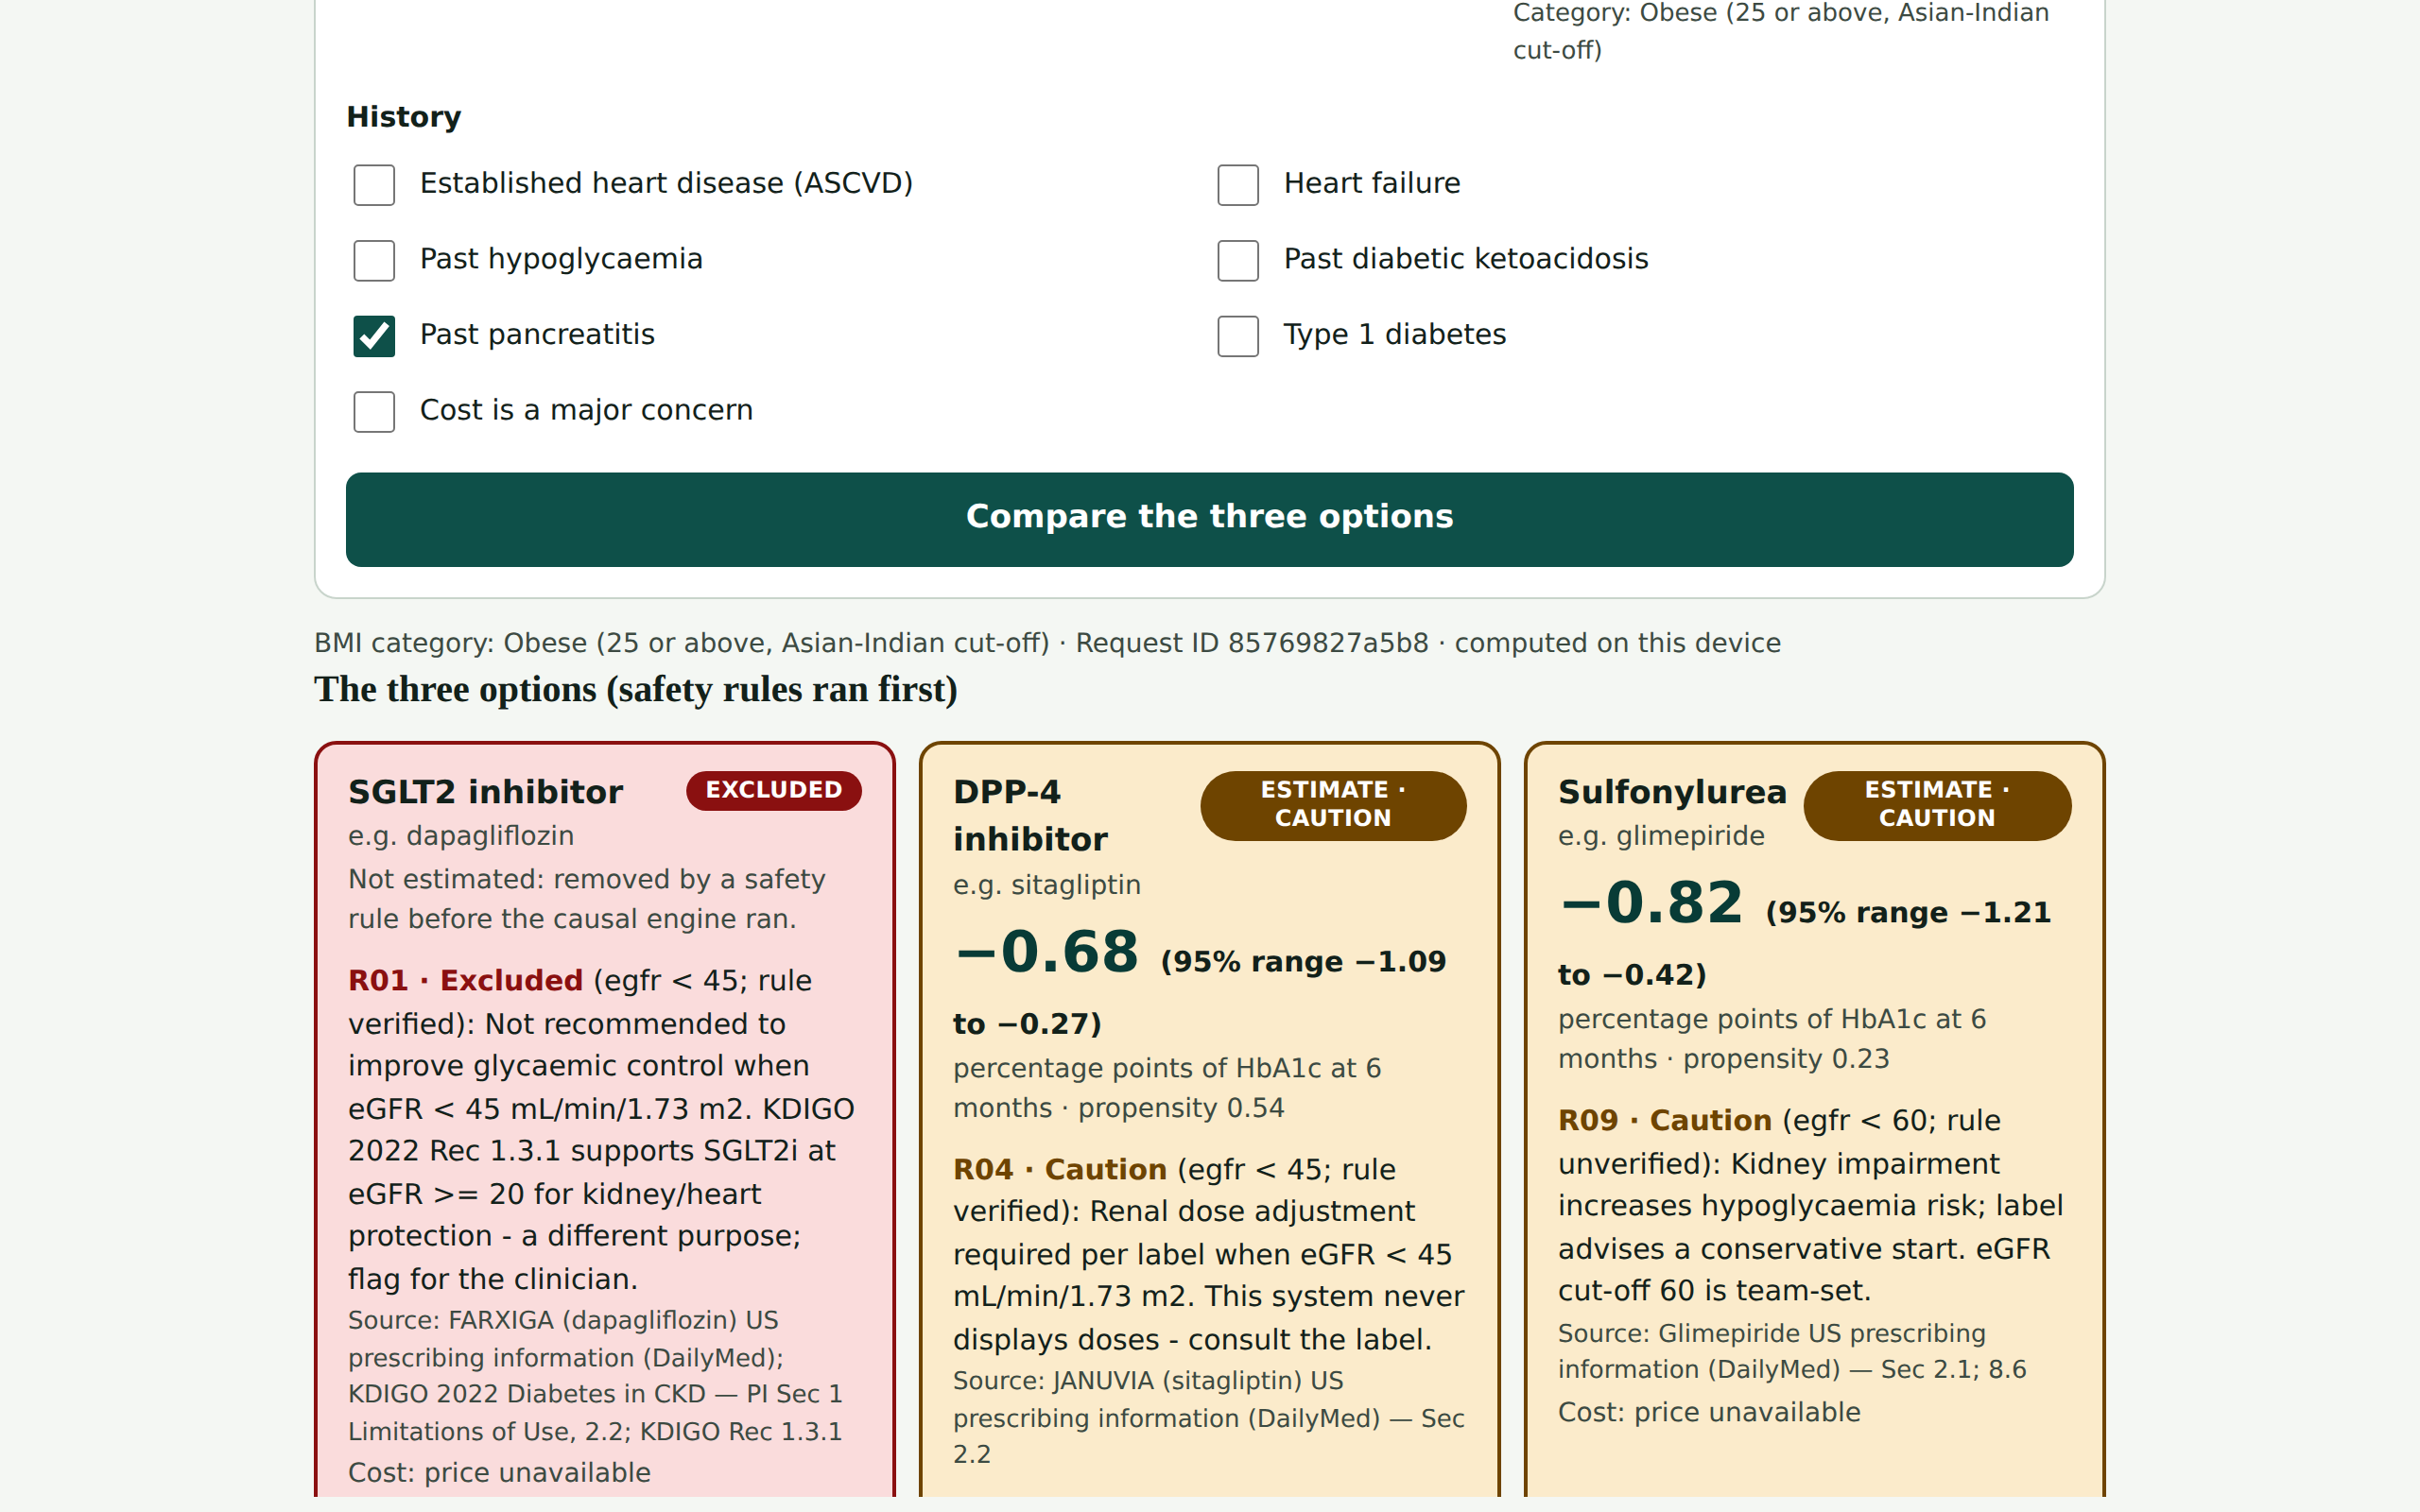
\includegraphics[width=0.95\textwidth]{screens/tryit_desktop.png}
\caption{Consultation screen: patient details, then the three options with exclusions, cautions and sources}\label{fig:ui}\end{figure}

\subsection{Block Diagram}
\begin{figure}[H]\centering
\resizebox{\ifdim\width>\textwidth\textwidth\else\width\fi}{!}{\begin{tikzpicture}[>=Stealth,font=\small,box/.style={draw,rounded corners,align=center,minimum height=0.9cm,inner sep=4pt}]
\node[box,minimum width=11.5cm,fill=gray!8] (ui) at (0,0) {User interface: phone website (Try it, Evidence, Results, Learn, About) \textbar\ Streamlit demo \textbar\ chat app};
\node[box,minimum width=3.6cm] (auth) at (-4,-1.6) {Accounts\\(sign-in, MFA, approval)};
\node[box,minimum width=3.6cm] (api) at (0.2,-1.6) {FastAPI service\\/api/v1/recommend};
\node[box,minimum width=3.2cm] (au) at (4.3,-1.6) {Audit log\\(no patient values)};
\node[box,minimum width=6cm] (g) at (-1.9,-3.2) {Safety rules engine (rules.csv, cited)};
\node[box,minimum width=6cm] (c) at (-1.9,-4.6) {Causal engine: propensity, overlap,\\AIPW, DR-learner, 95\% intervals};
\node[box,minimum width=6cm] (k) at (-1.9,-6.0) {Cost lookup (prices.csv, dated)};
\node[box,minimum width=3.4cm] (r) at (4.1,-4.6) {Evidence (RAG):\\BM25 + vector + fusion};
\node[box,minimum width=3.4cm] (cor) at (4.1,-6.0) {Licence-cleared\\corpus};
\draw[->] (ui) -- (auth); \draw[->] (ui) -- (api); \draw[->] (api) -- (au);
\draw[->] (api) -- (g); \draw[->] (g) -- (c); \draw[->] (c) -- (k);
\draw[->] ([xshift=1.4cm]api.south) -- ++(0,-0.62) -| (r.north); \draw[->] (cor) -- (r);
\end{tikzpicture}}
\caption{Block diagram of DiaCausal}\label{fig:block}\end{figure}
The website runs the same fitted model and the same evidence search inside the browser (exported from Python as \texttt{model.json} and \texttt{evidence.json}); automated tests check that the browser and Python give identical answers, so patient details never need to leave the device.
